\documentclass[10pt,letterpaper]{article}
\usepackage{times}
\usepackage{epsfig}
\usepackage{graphicx}
\usepackage{amsmath}
\usepackage{amssymb}
\usepackage{todonotes}
\usepackage{subcaption}
\captionsetup{compatibility=false}
\usepackage[margin=1.5in]{geometry}


% Include other packages here, before hyperref.

% If you comment hyperref and then uncomment it, you should delete
% egpaper.aux before re-running latex.  (Or just hit 'q' on the first latex
% run, let it finish, and you should be clear).
\usepackage[pagebackref=true,breaklinks=true,letterpaper=true,colorlinks,bookmarks=false]{hyperref}
%Introduction
%Related Work
%Model 
%%%Subsecs for the different contributions (dataset, learning rate, loss, lstm failures
%Results
%Discussion
%Conclusion

% \cvprfinalcopy % *** Uncomment this line for the final submission

\def\httilde{\mbox{\tt\raisebox{-.5ex}{\symbol{126}}}}

% Pages are numbered in submission mode, and unnumbered in camera-ready
%\ifcvprfinal\pagestyle{empty}\fi
\begin{document}

%%%%%%%%% TITLE
\title{Multimodal Classification of Lung Diseases}
\author{Felipe Moreno, Haripriya Mehta and Daniel Lee}

\maketitle

%\thispagestyle{empty}
%%%%%%%%% ABSTRACT
\begin{abstract}
We present a multimodal multi-class classification model that can recognize eight different types of lung diseases (infiltration, effusion, atelectasis, nodule, mass, pneumothorax, cardiomegaly and pneumonia). The model is multimodal because the features consists of not only chest X-ray images, but also patient age and gender. The model was trained on an imbalanced NIH Chest X-ray dataset, where each chest X-ray may have no disease, one disease, or multiple diseases. Through data augmentation, precision-recall tradeoff to achieve better generalization, our model is able to achieve a 0.7 global AUROC. We also show the precision of correctly predicting the presence of each individual disease, as well as AUROC for each individual disease.
\end{abstract}

%%%%%%%%% BODY TEXT
\section{Introduction and Related Work}

In the past decade, there has been incredible progress made in the area of computer vision through the development of deep learning and large-scale annotated image datasets. Large-scale image datasets, such as ImageNet, enabled researchers to have a a systematic way to evaluate their computer models \cite{Imagenet}. Deep learning has been useful in extracting complicated features from images using convolutional neural networks (CNN).

Deep learning has been similarly effective in medical image analysis. Some recent advances by using CNN include pulmonary nodule detection in CT images \cite{Pulmonary}, automated pancreas segmentation, \cite{Deeporgan}, and pinpointing spinal radiological scores \cite{Spinenet}. These advances are limited by the fact that the models are based on a limited datasets that consist of at most several hundred patients. As a result, from these studies alone, it has been unclear how well the deep learning models will scale to large-scale patient studies.

In order to tackle this issue, NIH has developed a new chest X-ray database, called "ChestX-ray8" in 2017 \cite{1705.02315}. The database consists of 108,948 frontal-view X-ray images of 32,717 patients from the year 1992 to 2015. Natural Language Processing was used to text-mine the common disease labels from each unique patients. Therefore, developing machine learning models for the dataset shows more promise of being useful to the greater patient populations.

Otherwise, the deep learning models for the ChestX-ray8 dataset has some practical uses. They can: (1) confirm radiologists' results and even identify diseases that may have been overlooked (2) identify slow changes in the patient's chest X-ray (3) be used in developing countries that lack radiologists (4) be applied to more complex dataset such as CT scans and MRI.

Wang et al., the the paper which introduces the ChestX-ray8 dataset, utilizes well established CNN \cite{1705.02315}. These CNN includes AlexNet, GoogLeNet, VGGNet-16, and ResNet-50. In the ChexNet paper released by Stanford (Rajpurkar et al.), which trains on the ChestX-ray 8 dataset, Stanford scientists use a 121-layer Dense CNN \cite{1711.05225} and achieve higher results than previous papers. In this paper, we go beyond the traditional CNN: we use multimodal deep learning model that takes both images and other patient features, such as gender and age, as inputs. Through this, we aim to increase the accuracy of our deep learning model.

\section{Dataset}
The NIH Chest dataset is a dataset that consists of chest X-rays images, patient age, and gender. 
The chest X-ray images is categorized into one or more of the 15 different classes - 14 of which are lung diseases (infiltration, effusion, atelectasis, nodule, mass, pneumothorax, consolidation, pleural thickening, cardiomegaly, emphysema, edema, fibrosis, pneumonia and hernia) and 1 of which is disease free.

Example of images found in the dataset are included in Figure \ref{dataset_example}.

\begin{figure}[h]
	\centering
	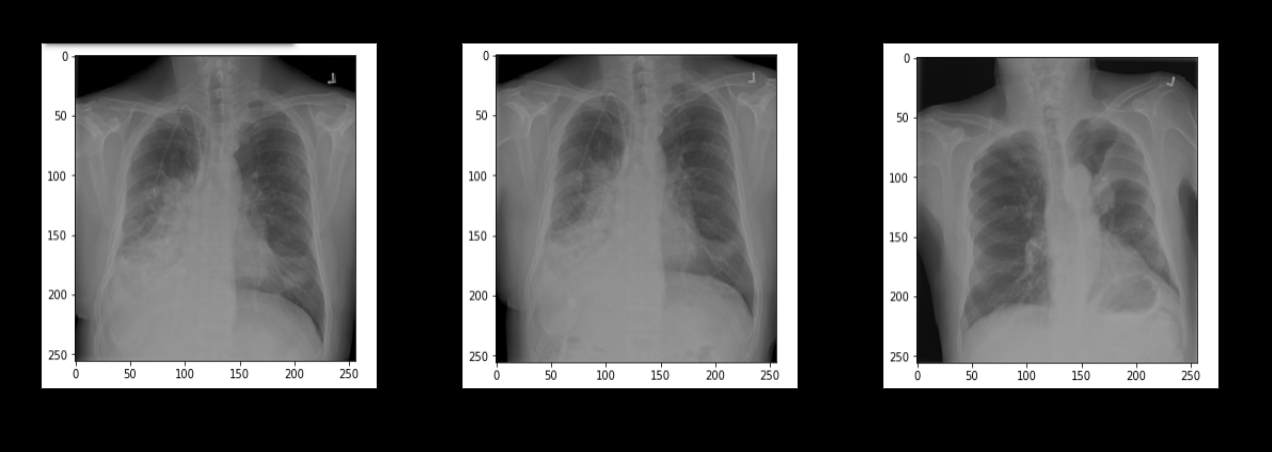
\includegraphics[scale=0.5]{./chestimages.png}
	\caption{Examples of chest X-rays found in the dataset.}
	\label{dataset_example}
\end{figure}

\subsection{Data pre-processing}
We first pre-process the data to ensure that we exclude any out of range values. For example, few of the patient ages were listed as 414, so we eliminated such rows. In Figure(\ref{class_distributions}), we display the distribution of the 15 different classes. 
\begin{figure}[htb]
	\centering
	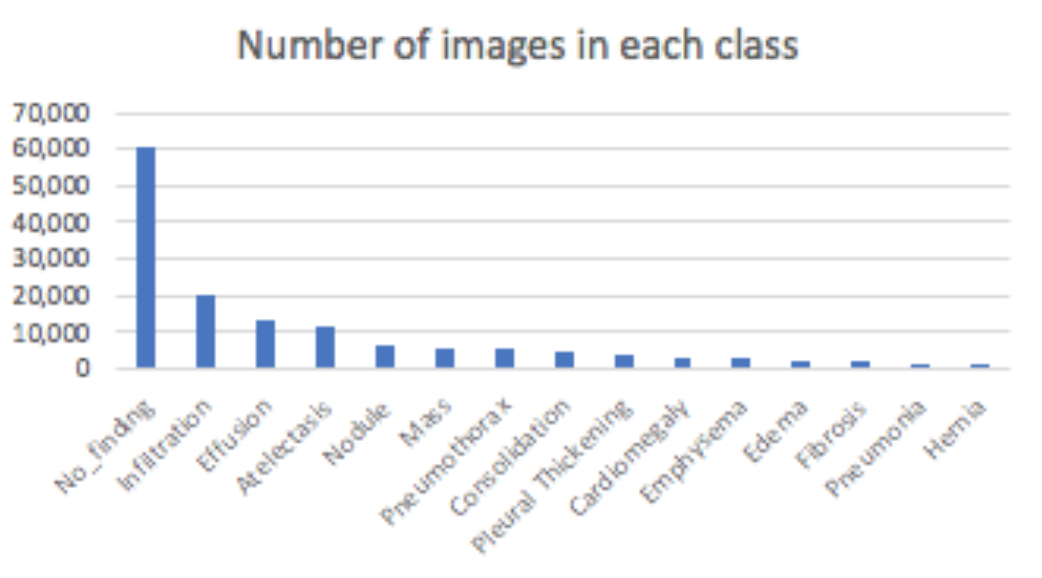
\includegraphics[width=\linewidth]{./imagedistribution.png}
	\caption{Dataset disease distributions}
	\label{class_distributions}
\end{figure}
\newline 

Due to severe under representation of data in certain categories, we limit ourselves to the eight disease categories that are found in Wang et al. \cite{1705.02315} : infiltration, effusion, atelectasis, nodule, mass, pneumothorax, cardiomegaly, and pneumonia. Each entry in the dataset contains an X-ray image and additional features, namely age and gender of the patient.  We divide the dataset into 60\% for the training set, 20\% for the validation set and 20\% for the test set. Each set is similarly distributed, as shown in Figure(\ref{dataset}).
\begin{figure}[htb]
	\centering
	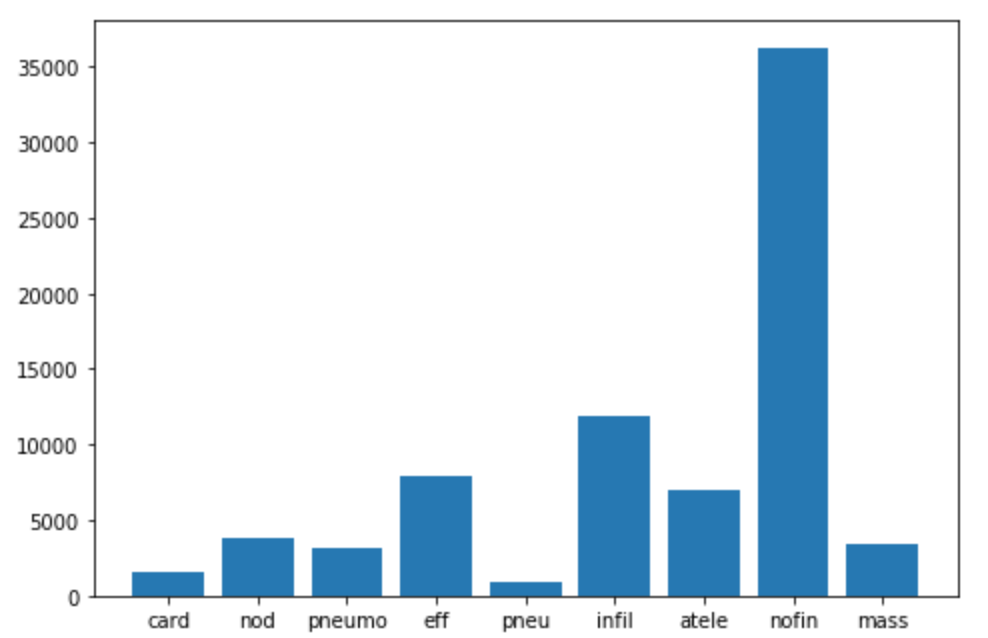
\includegraphics[width=0.3\linewidth]{./trainset.png}
	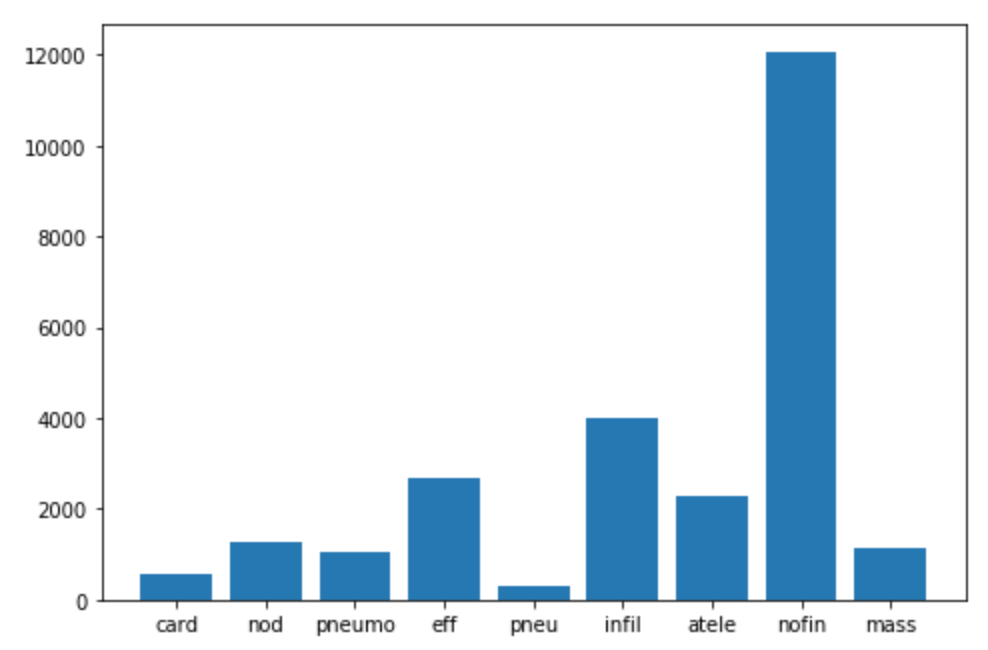
\includegraphics[width=0.3\linewidth]{./valset.png}
	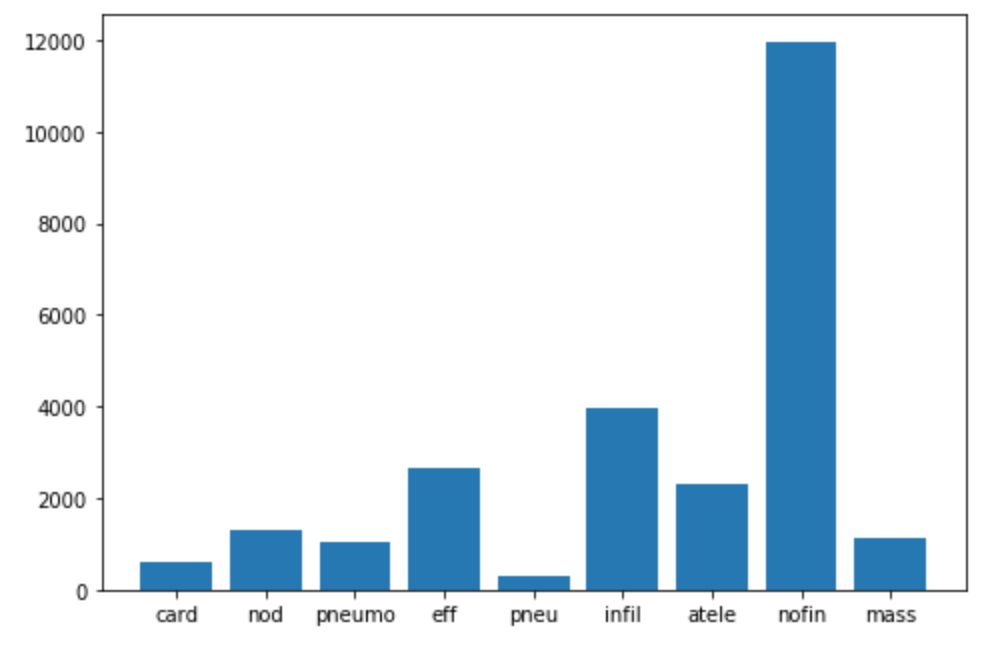
\includegraphics[width=0.3\linewidth]{./testset.png}
	\caption{From left to right: training set distribution, validation set distribution and test set distribution}
	\label{dataset}
\end{figure}

\section{Model}
Our model takes advantage of the additional features provided in the dataset, age and gender, which are discretized into a length 12 vector using a one-hot encoding. The first two positions in the vector represent male and female. The last ten positions represent age intervals [1-10], [11-20], ..., [91-100]. For example, the one-hot encoding of [1, 0, 0, 0, 0, 1, 0, 0, 0, 0, 0, 0] encodes a male patient aged between 31-40 years.

Our model features a CNN with X-ray images as input. The CNN outputs are then passed to a Fully Connected (FC) layer Figure(\ref{architecture}). The additional features are also passed to a FC layer, and the two FC layers are concatenated to each other. Then, there are two additional FC layers. The last FC layer outputs eight nodes through the sigmoid function, with each node representing each disease.

\begin{figure}[h]
	\centering
	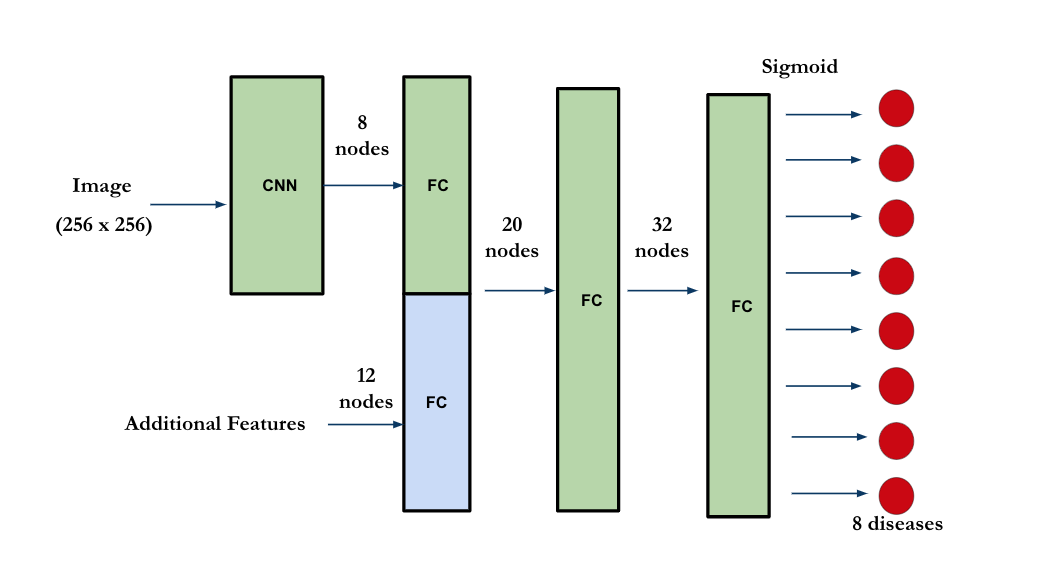
\includegraphics[scale=0.7]{./model_image.png}
	\caption{Multi-modal Model Architecture}
	\label{architecture}
\end{figure}

\subsection{CNN}
We experiment with different state-of-the art models for the CNN, such as VGGNet, AlexNet and ResNet. We defined the CNN output to be 8 nodes - each node representing a different disease. We used this CNN architectures as a baseline model to compare against the multi-modal model. Wang et al. used AlexNet, GoogLeNet, VGGNet-16, and ResNet-50 as their CNN model \cite{1705.02315}. However, the results from the paper will not be used as the baseline because they likely had much more resources than we do. In order to have a comparison between CNN-only and multi-modal models with minimum confounding factors, we ran both ourselves.

\subsection{Precision - Recall balancing}
Since most of the data points contain no diseases, without properly balancing precision and recall, the model would tend to predict a datapoint to have no disease. This decision may be great in terms of accuracy, but the recall would be low. We tackle this issue at the loss criteria formulation. By setting the parameters called 'pos weights' of the loss function, we can trade off between recall and precision. For each disease class we set the 'pos weight' parameter to be greater than 1. This decreases the false negative count, increasing recall as a result. For each diseases class $i$ we set 
$$ \text{pos weight}_i = \frac{\text{numer of negative labeled points for disease i}}{\text{number  of positively labeled points for disease i}}$$
In this way, we effectively balance the labels for each class. 

\subsection{Loss Function}
The loss function is a Binary Cross Entropy Loss with Logits. This is a featured loss function in Pytorch which first filters the outputs of the model through a sigmoid function and then uses these values to compute the binary cross entropy for each classification label. We chose this loss function because it is appropriate for a multi-class classification problem: data points may contain no disease, one disease or multiple diseases. For this reason, we chose a loss function that is capable of outputting a probability of each disease being present in the datapoint.

\section{Metrics}
We used Receiver Operating Characteristic (ROC) Area Under the Curve (AUC) to measure the accuracy of the model. This metric assesses the capability of the model to distinguish between different classes, and has been used in the past to validate X-Ray images in the ChexNet paper \cite{1711.05225}. 

We calculate the global ROC AUC statistic by counting the total of true positives, false negatives and false positives. During training, we use the global ROC AUC statistic to find the model that best generalizes. Then we use the validation set to confirm the capabilities of the model. We also report the model's breakdown of ROC AUC per disease.

\section{Experiments}

\subsection{Architecture}
We first trained on standard CNN architectures and then compared their predictions to our multimodal model. We used VGG, Resnet, and Alexnet with different depths.

\subsection{Optimizer}
In our experiments, we used the stochastic gradient descent optimizer with a step scheduler to tune the learning rate as the loss decreased. Through trial and error, we found that setting an initial learning rate of 0.01 and updating the learning rate by a factor of 0.1 every 10 epochs minimized the loss function smoothly.

\subsection{Data augmentation}
In the first set of experiments, both the pure CNN model and the multi-modal model started to overfit around the 15th epoch. By looking at the actual images, we observed that the images were highly irregular, as seen in Figure(\ref{image_irregularities}). Some of the images were tilted, while other X-rays only showed the thorax. Other images were more zoomed out or were shifted upwards, partially displaying the abdomen. Some images partially displayed the skull.

In order to improve the generalization of the model, we performed data augmentation on the training set. With probability 0.5, we performed one random operation from the following: rotating by $\pm 15^\circ$, scaling by a random factor between (0.1, 0.15), translating by a maximum factor of 0.2 in each x and y directions, or reflecting horizontally.


\begin{figure}[]
	\begin{tabular}[c]{ccc}
		\begin{subfigure}[c]{0.3\textwidth} 
			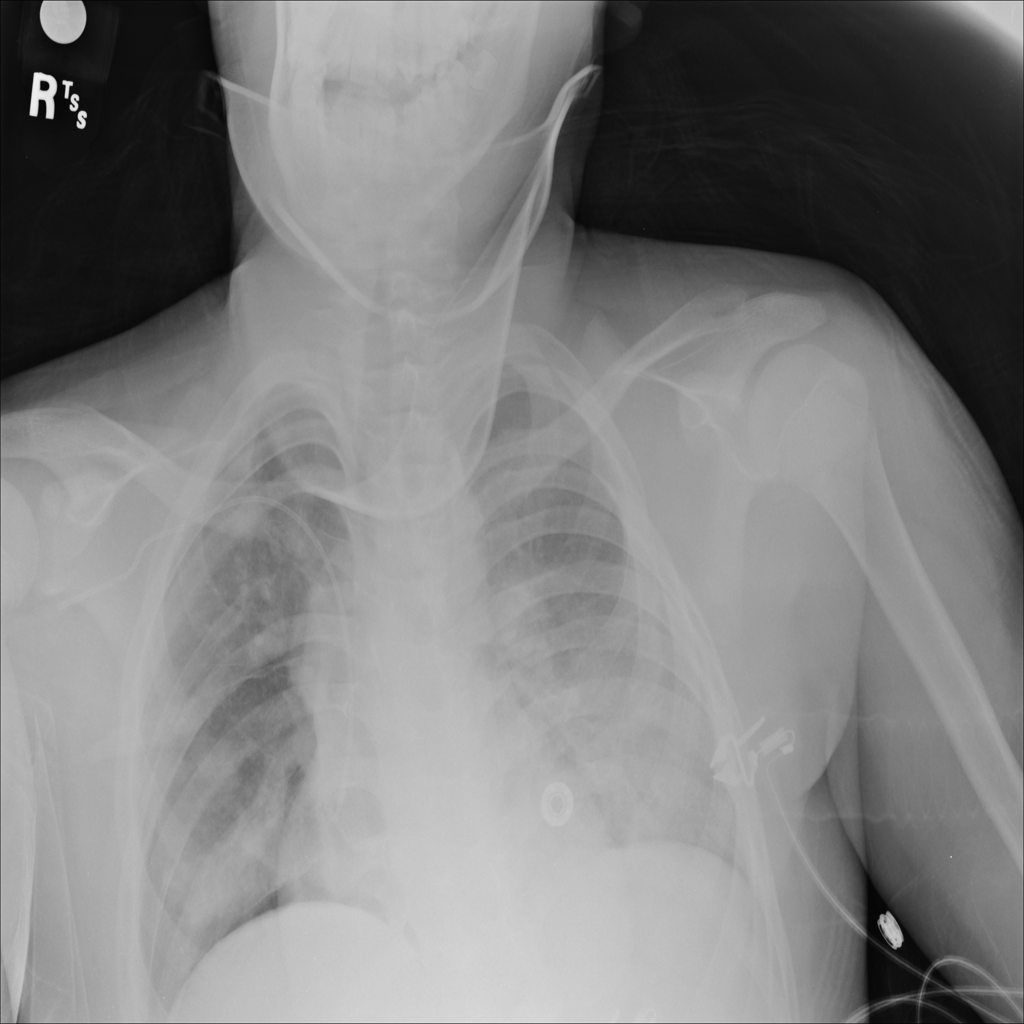
\includegraphics[width=\linewidth]{./skull.png}
			\subcaption{Image contains regions of the skull}
		\end{subfigure}&
		\begin{subfigure}[c]{0.3\textwidth}
			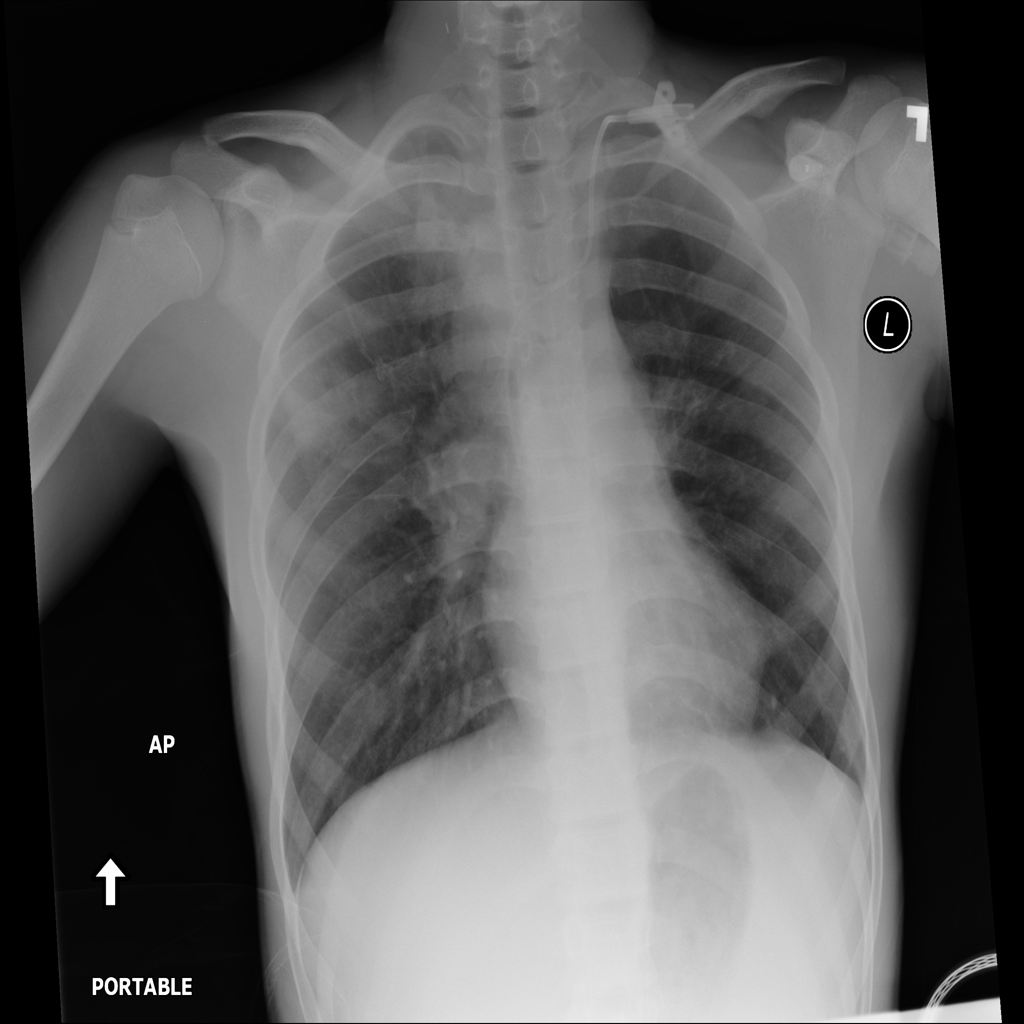
\includegraphics[width=\linewidth]{./shifted_right.png}
			\subcaption{Image contains regions of the abdomen}
		\end{subfigure}&
		\begin{subfigure}[c]{0.3\textwidth}
			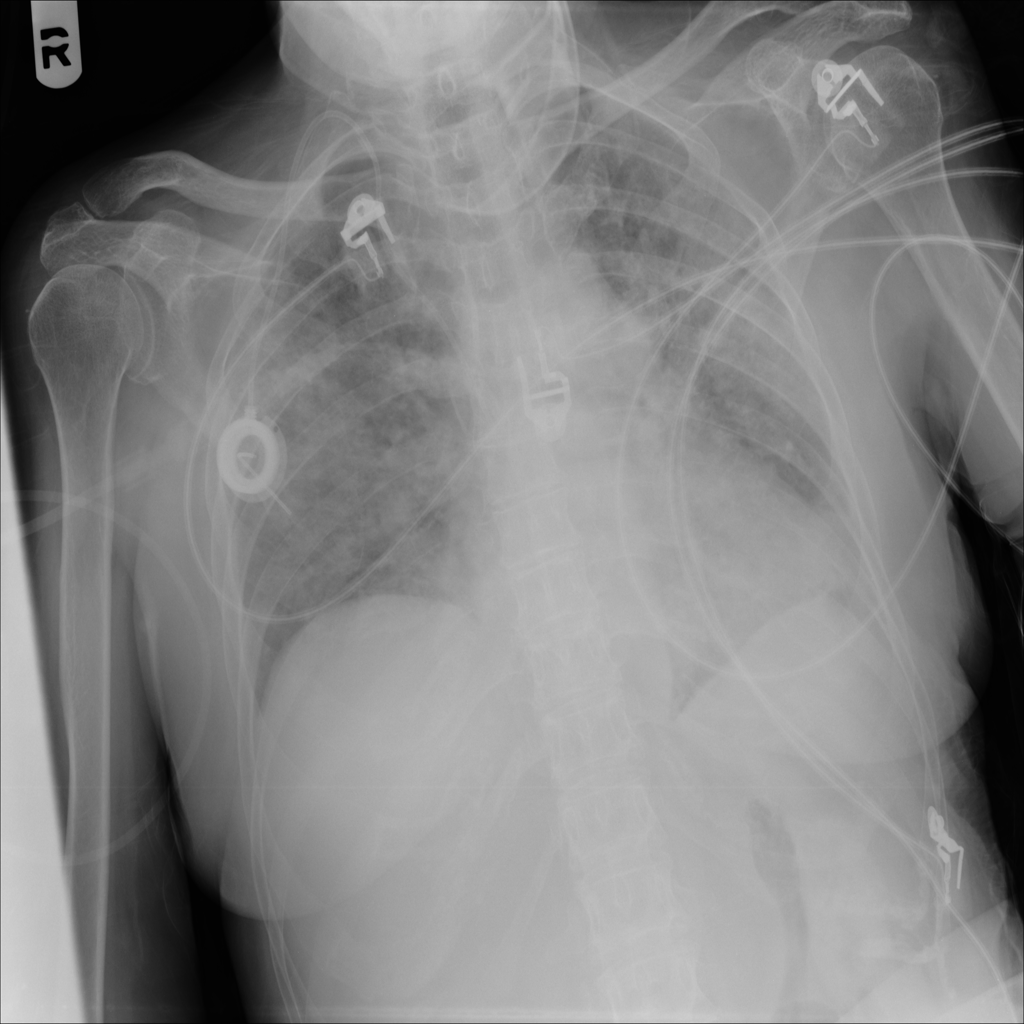
\includegraphics[width=\linewidth]{./tilted.png}
			\subcaption{Image is tilted counterclockwise.}
		\end{subfigure}
	\end{tabular}
	\caption{Irregular image samples.}
	\label{image_irregularities}
\end{figure}

\subsection{Going deeper}
We tried training deeper models using ResNet-34 and ResNet-50. 
From around 15 epochs, the multi-modal model started to overfit, even with data augmentation. Therefore, we tried to add the dropout layers with probability 0.5 after the non-linearities of the last two fully connected layers in hopes to further regularize learning.

\section{Results}
For the pure-CNN models, VGG had a poor performance and failed to properly fit the data from just one epoch. Although Alexnet performed relatively good results for a shallow network, it was unable to capture the complexity of the dataset. With data augmentation, Resnet-18 was able to train without overfitting and converged to the best validation ROC AUC of 0.7245, shown in  Table(\ref{roc}).

\begin{table}[!htbp]
\centering
\begin{tabular}{| l | l | l | l | l}
\hline
           & \textbf{Loss}   & \textbf{Accuracy} (\%) & \textbf{ROC AUC} \\ \hline
\textbf{Training}   & 0.8662 & 74.6587       & 0.7452 \\ \hline
\textbf{Validation} & 1.0886 & 76.0343       & 0.7245\\ \hline
\end{tabular}
\caption{Training and Validation Loss, Accuracy and global ROC AUC with CNN (Resnet-18)}
\label{roc}
\end{table}

We used the Resnet-18 as a benchmark for CNN, and continued to experiment with the multi-modal model. Even with data augmentation using ResNet-50, the multimodal could only achieve a best validation ROC AUC of 0.6954. The results are shown in Table(\ref{resnet50}).

\begin{table}[!htbp]
\centering
\begin{tabular}{| l | l | l | l | l}
\hline
           & \textbf{Loss}   & \textbf{Accuracy} (\%) & \textbf{ROC AUC} \\ \hline
\textbf{Training}   & 0.9460 & 69.9630       & 0.7047 \\ \hline
\textbf{Validation} & 1.1647 & 71.9971       & 0.6973\\ \hline
\end{tabular}
\caption{Training and Validation Loss, Accuracy and global ROC AUC with multi-modal  model (resnet-50)}
\label{resnet50}
\end{table}

Lastly, we display the ROC AUC per disease for our best model (pure CNN, Resnet-18) in Table (\ref{perdisease}). We compare the model to the best result found in literature (CheXNet) \cite{1711.05225}. 

\begin{table}[!htbp]
\centering
\begin{tabular}{|l|l|l|}
\hline
\textbf{Disease}      & \textbf{Our ROC AUC} & \textbf{ChexNet ROC AUC} \\ \hline
Cardiomegaly & 0.811 & 0.925\\ \hline
Nodule       & 0.622 & 0.780\\ \hline
Pneumothorax & 0.765 & 0.888\\ \hline
Effusion     & 0.781 & 0.864\\ \hline
Pneumonia    & 0.628 & 0.768\\ \hline
Infiltration & 0.633 & 0.735\\ \hline
Atelectasis  & 0.707 & 0.809\\ \hline
Mass         & 0.719 & 0.868\\ \hline
\end{tabular}
\caption{ROC AUC per disease for test data}
\label{perdisease}
\end{table}



\section{Criticism}
The disease state was collected using NLP techniques from the patients data \cite{1705.02315}. There were no radiologists that actually looked at and labelled the X-ray images, nor were there efforts made to corroborate the quality of the images Figure (6). As a result, machine learning specialist and radiologist Luke Oakden-Rayner \cite{luke} claims that a lot of the X-ray images from the Chest-Xray8 are actually mis-classified. In many of the successful papers such as the ChexNet paper \cite{1711.05225}, professional radiologists relabeled their dataset.

\begin{figure}[ht]
	\begin{tabular}[c]{ccc}
		\begin{subfigure}[c]{0.3\textwidth} 
			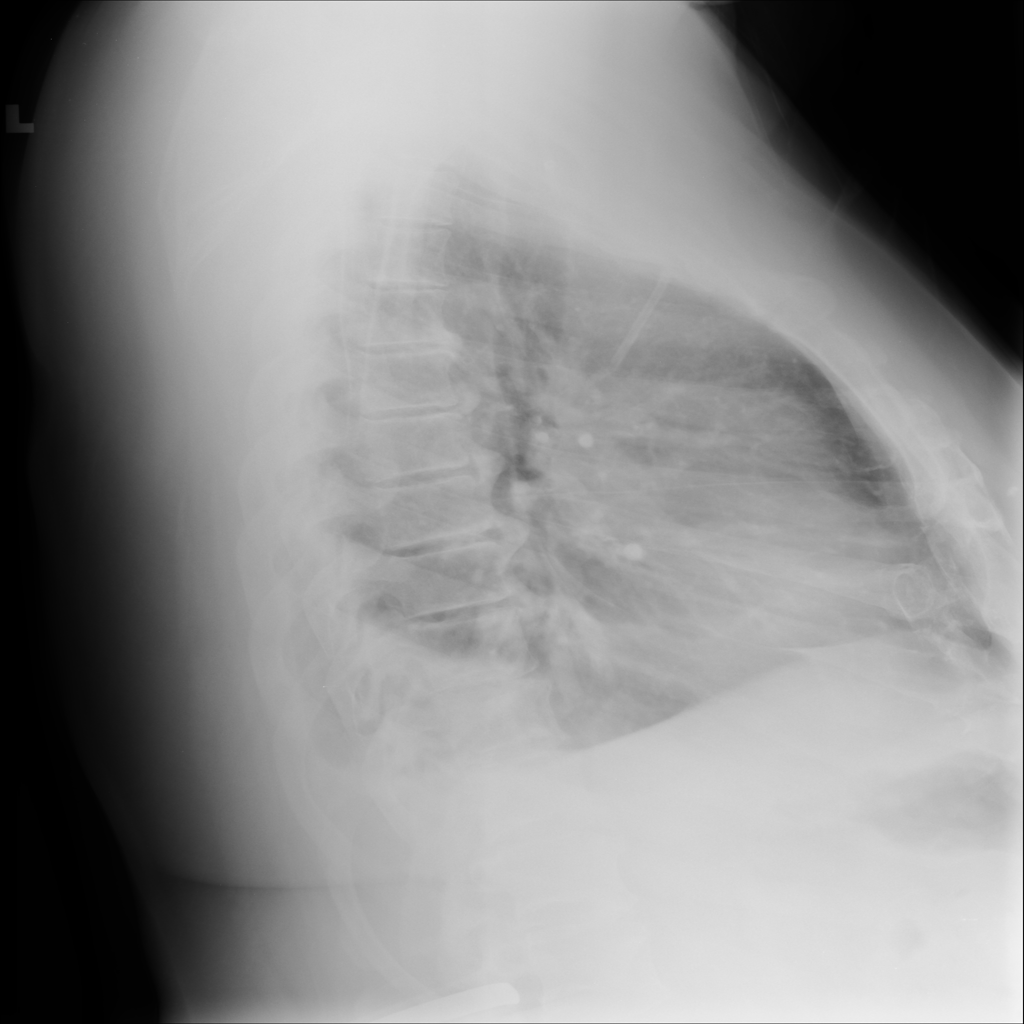
\includegraphics[width=\linewidth]{./outcast.png}
			\subcaption{Image is not front chest}
		\end{subfigure}&
		\begin{subfigure}[c]{0.3\textwidth}
			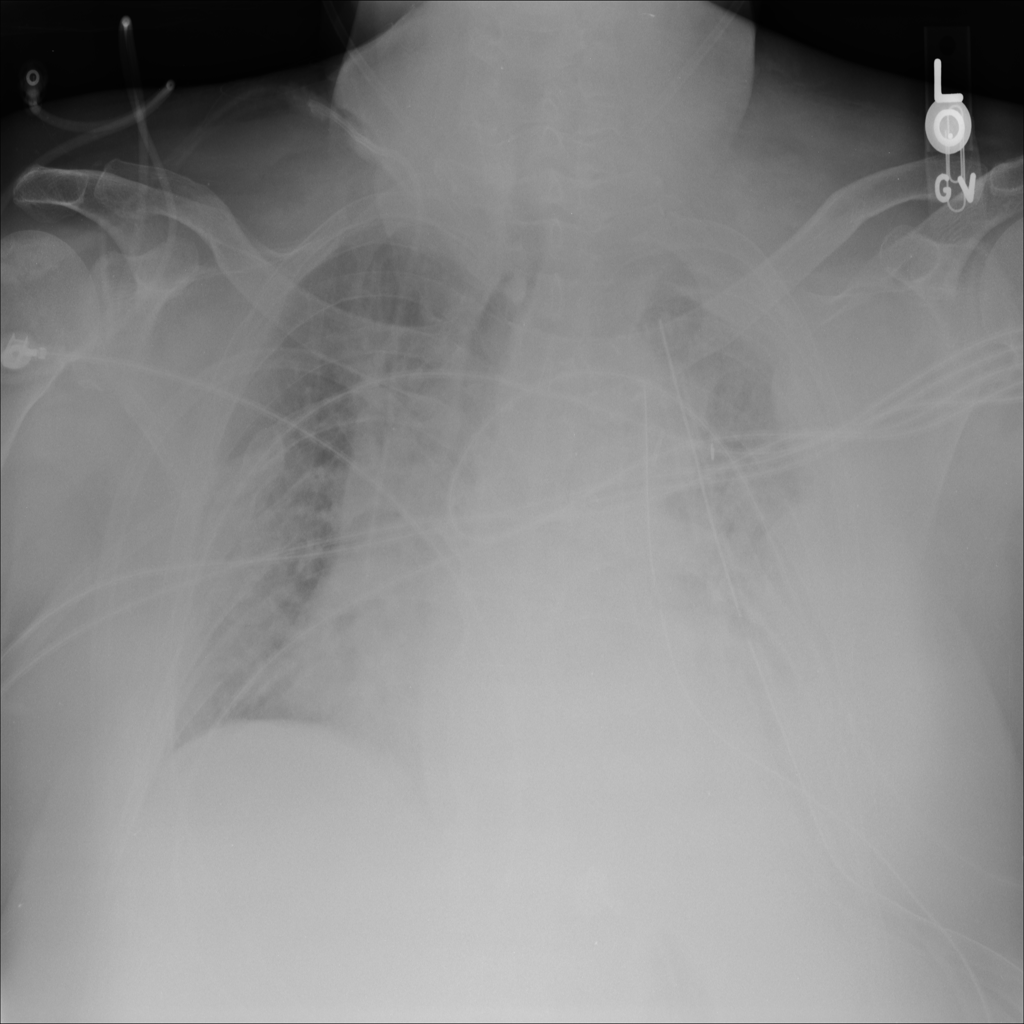
\includegraphics[width=\linewidth]{./distorted1.png}
			\subcaption{Image is highly distorted}
		\end{subfigure}&
		\begin{subfigure}[c]{0.3\textwidth}
			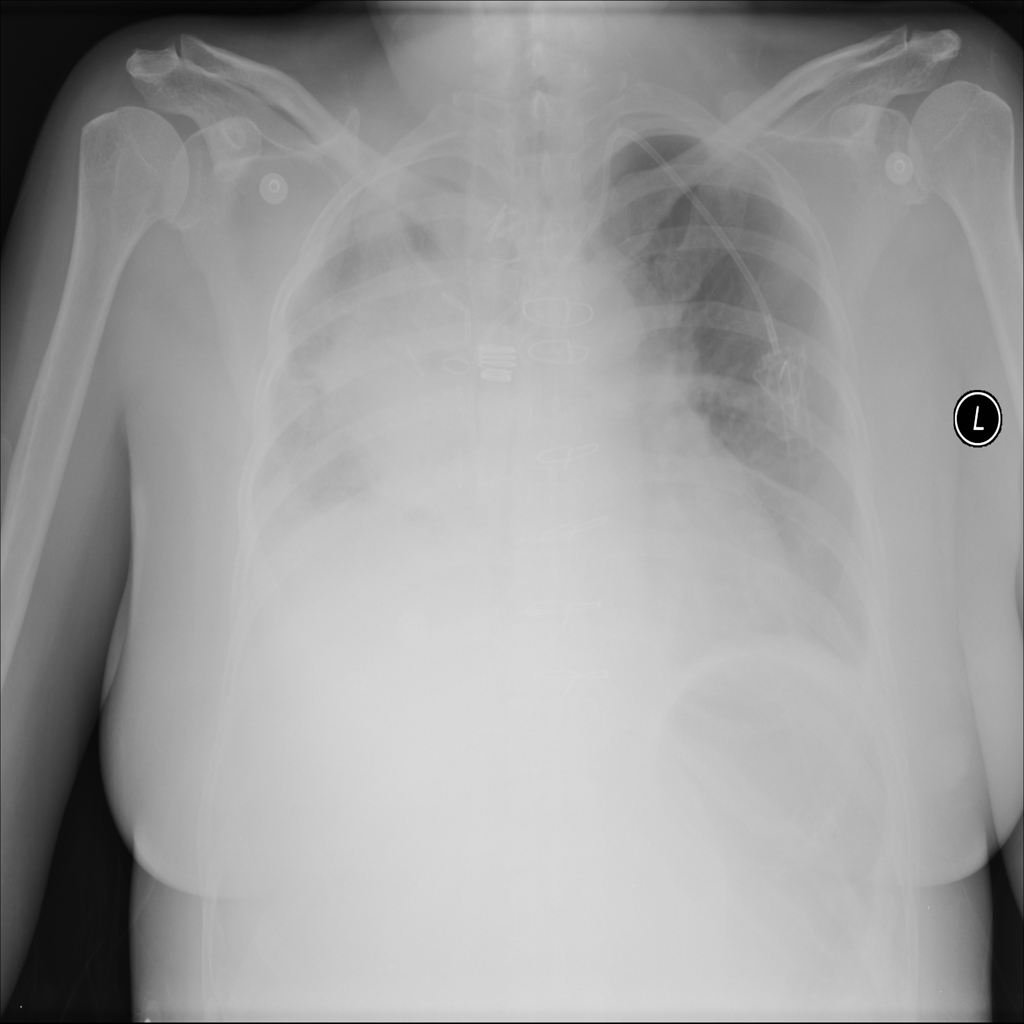
\includegraphics[width=\linewidth]{./distorted2.png}
			\subcaption{Image is highly distorted}
		\end{subfigure}
	\end{tabular}
	\caption{Dataset irregularities }
	\label{outcast}
\end{figure}

\section{Conclusion \& Future Work}

In conclusion, our multi-modal model fails to outperform the pure-CNN model. Moreover, our best model's ROC AUC was not as high as that from the Stanford's CheXNet paper.
The paper has a significant advantage, however, of being relabelled correctly by radiologists. In the future, we expect improve our ROC AUC of our multi-modal dataset by training on medical datasets that have more features than just patient age and gender.

\section{Appendix}

\subsection{Other attempts}

The way that our additional features was set up was not the most appropriate way to do it. We were encoding the same piece of information (gender) in two different positions. This can cause a dummy variable trap. Furthermore, in the medical world, equal intervals of ages may not represent equal likelihood of obtaining disease - a 31 may be very different from a 38 year old. 

Keeping all other things constant, we modify our additional features to be a length 2 vector. The
first position in the vector represents male (1) and female (0). The second position represents the normalized age (age/100). 

However, after redoing experiments on ResNet-50, we obtained a global AUC ROC of 0.5 and per-disease AUC ROC of 0.5, which means that our prediction is as good as a random guess.

We believe that given more time, by modifying the model to account for the change in features, we could have obtained better results. 

\subsection{Division of Labor}

All of the members contributed to each of the parts. Special acknowledgement is made to Felipe for setting up the GPU environment to design and train the experiments, and tackling the multi-class and data imbalance problem; Haripriya for looking into multi-modal neural networks and creating most of the presentation; and Daniel for finding the project to work on and leading the data pre-processing.


\bibliographystyle{unsrt}
\bibliography{egbib.bib}

\end{document}

%------------------------------------------------------------------------




%------------------------------------------------------------------------


